\documentclass[12pt,a4paper]{article}
\usepackage[utf8]{inputenc}
\usepackage[left=1in,right=1in,top=1in,bottom=1in]{geometry}

\author{May Helena Plumb}
\title{Encoding Ticha Documents with TEI/XML}

\makeatletter
\let\thetitle\@title
\let\theauthor\@author
\makeatother

\usepackage{marginnote}

\usepackage{graphicx}

\usepackage[usenames, dvipsnames]{color}
 
\definecolor{codegreen}{rgb}{0,0.54,0}
\definecolor{codegray}{rgb}{0.5,0.5,0.5}
\definecolor{codepurple}{rgb}{0.38,0,0.62}
\definecolor{backcolour}{rgb}{1.0,1.0,1.0}
\definecolor{codeyellow}{rgb}{0.75,0.54,0.13}
\definecolor{codered}{rgb}{0.54,0.0,0.0}
\definecolor{codeblue}{rgb}{0.0,0.0,0.54}


%\usepackage[T1]{fontenc} % straight quotes

\usepackage{textcomp}
\usepackage{listings}

 
\lstdefinestyle{mystyle}{
    language=XML,
    backgroundcolor=\color{backcolour},
    tagstyle=\color{codeblue},
    commentstyle=\color{codegreen},
    keywordstyle=\color{codeyellow},
    morekeywords={xml:id,type,break,facs,n,org,sample,part},
    numberstyle=\tiny\color{codegray},
    stringstyle=\color{codered},
    basicstyle=\footnotesize\ttfamily,
    breakatwhitespace=false,         
    breaklines=true,                 
    captionpos=b,                    
    keepspaces=true,                 
    numbers=left,                    
    numbersep=5pt,                  
    showspaces=false,                
    showstringspaces=false,
    showtabs=false,                  
    tabsize=2,
    escapechar=^
}
 
\lstset{style=mystyle}

\newcommand{\keyword}[1]{\textbf{#1}}

\newcommand{\taglinks}[2]{
\vspace*{-0.5ex}
\hspace*{\parindent}
\begin{minipage}{\textwidth}
  \emph{Possible attributes: #1.} \\ \url{#2} \end{minipage} \vspace{0.5ex} \\ }


%\usepackage{url}

\usepackage{soul}

\usepackage{hyperref}
\hypersetup{
    colorlinks=true,
    linkcolor=blue,
    filecolor=magenta,      
    urlcolor=codepurple,
   % bookmarks=true,
   %hyperindex=true,
}


\begin{document}

Issues:
\begin{itemize}
\item are we using \texttt{<hi>} correctly?
\item should we have used the part attribute for paragraphs?
\end{itemize}

\begin{center}
{\large \textbf{\thetitle}} \\
Guidelines by \theauthor \\
\emph{last updated \today}
\end{center}

\tableofcontents	

%Introduction information...

%\begin{lstlisting}
%<?xml version="1.0" encoding="UTF-8"?><?xml-model href="TEISchema_current.rnc" type="application/relax-ng-compact-syntax"?>
%<TEI xmlns="http://www.tei-c.org/ns/1.0" xml:space="preserve">
%\end{lstlisting}

\section{About this Documentation}

\section{Tags}

\subsection{TEI Prelude}

\subsubsection{\texttt{<TEI>}} \label{tag-sec:TEI}
\taglinks{
\hyperref[att-sec:xxx]{\texttt{xxx}}, ... }
{http://www.tei-c.org/release/doc/tei-p5-doc/en/html/ref-TEI.html}
This tag...

\subsubsection{\texttt{<teiHeader>}} \label{tag-sec:teiHeader}
\taglinks{
\hyperref[att-sec:xxx]{\texttt{xxx}}, ... }
{http://www.tei-c.org/release/doc/tei-p5-doc/en/html/ref-teiHeader.html}
This tag... (marked as deprecated)

\subsubsection{\texttt{<fileDesc>}} \label{tag-sec:fileDesc}
\taglinks{
\hyperref[att-sec:xxx]{\texttt{xxx}}, ... }
{http://www.tei-c.org/release/doc/tei-p5-doc/en/html/ref-fileDesc.html}
This tag...

\subsubsection{\texttt{<titleStmt>}} \label{tag-sec:titleStmt}
\taglinks{
\hyperref[att-sec:xxx]{\texttt{xxx}}, ... }
{http://www.tei-c.org/release/doc/tei-p5-doc/en/html/ref-titleStmt.html}
This tag...

\subsubsection{\texttt{<title>}} \label{tag-sec:title}
\taglinks{
\hyperref[att-sec:xxx]{\texttt{xxx}}, ... }
{http://www.tei-c.org/release/doc/tei-p5-doc/en/html/ref-title.html}
This tag...

\subsubsection{\texttt{<publicationStmt>}} \label{tag-sec:publicationStmt}
\taglinks{
\hyperref[att-sec:xxx]{\texttt{xxx}}, ... }
{http://www.tei-c.org/release/doc/tei-p5-doc/en/html/ref-publicationStmt.html}
This tag...

\subsubsection{\texttt{<profileDesc>}} \label{tag-sec:profileDesc}
\taglinks{
\hyperref[att-sec:xxx]{\texttt{xxx}}, ... }
{http://www.tei-c.org/release/doc/tei-p5-doc/en/html/ref-profileDesc.html}
This tag...

\subsubsection{\texttt{<encodingDesc>}} \label{tag-sec:encodingDesc}
\taglinks{
\hyperref[att-sec:xxx]{\texttt{xxx}}, ... }
{http://www.tei-c.org/release/doc/tei-p5-doc/en/html/ref-encodingDesc.html}
This tag...

\subsubsection{\texttt{<sourceDesc>}} \label{tag-sec:sourcesDesc}
\taglinks{
\hyperref[att-sec:xxx]{\texttt{xxx}}, ... }
{http://www.tei-c.org/release/doc/tei-p5-doc/en/html/ref-sourceDesc.html}
This tag...

\subsubsection{\texttt{<langUsage>}} \label{tag-sec:langUsage}
\taglinks{
\hyperref[att-sec:xxx]{\texttt{xxx}}, ... }
{http://www.tei-c.org/release/doc/tei-p5-doc/en/html/ref-langUsage.html}
This tag...

\subsubsection{\texttt{<language>}} \label{tag-sec:language}
\taglinks{
\hyperref[att-sec:xxx]{\texttt{xxx}}, ... }
{http://www.tei-c.org/release/doc/tei-p5-doc/en/html/ref-language.html}
This tag...

\subsubsection{\texttt{<projectDesc>}} \label{tag-sec:projectDesc}
\taglinks{
\hyperref[att-sec:xxx]{\texttt{xxx}}, ... }
{http://www.tei-c.org/release/doc/tei-p5-doc/en/html/ref-projectDesc.html}
This tag...

\subsubsection{\texttt{<editorialDecl>}} \label{tag-sec:editorialDecl}
\taglinks{
\hyperref[att-sec:xxx]{\texttt{xxx}}, ... }
{http://www.tei-c.org/release/doc/tei-p5-doc/en/html/ref-editorialDecl.html}
This tag...

\subsubsection{\texttt{<correction>}} \label{tag-sec:correction}
\taglinks{
\hyperref[att-sec:xxx]{\texttt{xxx}}, ... }
{http://www.tei-c.org/release/doc/tei-p5-doc/en/html/ref-correction.html}
This tag...

\subsubsection{\texttt{<normalization>}} \label{tag-sec:normalization}
\taglinks{
\hyperref[att-sec:xxx]{\texttt{xxx}}, ... }
{http://www.tei-c.org/release/doc/tei-p5-doc/en/html/ref-normalization.html}
This tag...

\subsubsection{\texttt{<hyphenation>}} \label{tag-sec:hyphenation}
\taglinks{
\hyperref[att-sec:xxx]{\texttt{xxx}}, ... }
{http://www.tei-c.org/release/doc/tei-p5-doc/en/html/ref-hyphenation.html}
This tag...

\subsubsection{\texttt{<segmentation>}} \label{tag-sec:segmentation}
\taglinks{
\hyperref[att-sec:xxx]{\texttt{xxx}}, ... }
{http://www.tei-c.org/release/doc/tei-p5-doc/en/html/ref-segmentation.html}
This tag...

\subsubsection{\texttt{<interpretation>}} \label{tag-sec:interpretation}
\taglinks{
\hyperref[att-sec:xxx]{\texttt{xxx}}, ... }
{http://www.tei-c.org/release/doc/tei-p5-doc/en/html/ref-interpretation.html}
This tag...

\subsubsection{\texttt{<refsDecl>}} \label{tag-sec:refsDecl}
\taglinks{
\hyperref[att-sec:xxx]{\texttt{xxx}}, ... }
{http://www.tei-c.org/release/doc/tei-p5-doc/en/html/ref-refsDecl.html}
This tag...

\subsubsection{\texttt{<cRefPattern>}} \label{tag-sec:cRefPattern}
\taglinks{
\hyperref[att-sec:xxx]{\texttt{xxx}}, ... }
{http://www.tei-c.org/release/doc/tei-p5-doc/en/html/ref-cRefPattern.html}
This tag...

\subsubsection{\texttt{<charDecl>}} \label{tag-sec:charDecl}
\taglinks{
\hyperref[att-sec:xxx]{\texttt{xxx}}, ... }
{http://www.tei-c.org/release/doc/tei-p5-doc/en/html/ref-charDecl.html}
This tag...

\subsubsection{\texttt{<glyph>}} \label{tag-sec:glyph}
\taglinks{
\hyperref[att-sec:xxx]{\texttt{xxx}}, ... }
{http://www.tei-c.org/release/doc/tei-p5-doc/en/html/ref-glyph.html}
This tag...

\subsubsection{\texttt{<glyphName>}} \label{tag-sec:glyphName}
\taglinks{
\hyperref[att-sec:xxx]{\texttt{xxx}}, ... }
{http://www.tei-c.org/release/doc/tei-p5-doc/en/html/ref-glyphName.html}
This tag...

\subsubsection{\texttt{<figure>}} \label{tag-sec:figure}
\taglinks{
\hyperref[att-sec:xxx]{\texttt{xxx}}, ... }
{http://www.tei-c.org/release/doc/tei-p5-doc/en/html/ref-figure.html}
This tag...

\subsubsection{\texttt{<graphic>}} \label{tag-sec:graphic}
\taglinks{
\hyperref[att-sec:xxx]{\texttt{xxx}}, ... }
{http://www.tei-c.org/release/doc/tei-p5-doc/en/html/ref-graphic.html}
This tag...

\subsubsection{\texttt{<add>}} \label{tag-sec:add}
\taglinks{
\hyperref[att-sec:xxx]{\texttt{xxx}}, ... }
{http://www.tei-c.org/release/doc/tei-p5-doc/en/html/ref-add.html}
This tag...

\subsubsection{\texttt{<c>}} \label{tag-seccTEI}
\taglinks{
\hyperref[att-sec:xxx]{\texttt{xxx}}, ... }
{http://www.tei-c.org/release/doc/tei-p5-doc/en/html/ref-c.html}
This tag...

\subsubsection{\texttt{<del>}} \label{tag-sec:del}
\taglinks{
\hyperref[att-sec:xxx]{\texttt{xxx}}, ... }
{http://www.tei-c.org/release/doc/tei-p5-doc/en/html/ref-del.html}
This tag...

\subsubsection{\texttt{<ptr>}} \label{tag-sec:ptr}
\taglinks{
\hyperref[att-sec:xxx]{\texttt{xxx}}, ... }
{http://www.tei-c.org/release/doc/tei-p5-doc/en/html/ref-ptr.html}
This tag...

\subsubsection{\texttt{<ref>}} \label{tag-sec:ref}
\taglinks{
\hyperref[att-sec:xxx]{\texttt{xxx}}, ... }
{http://www.tei-c.org/release/doc/tei-p5-doc/en/html/ref-ref.html}
This tag...

\subsubsection{\texttt{<g>}???} \label{tag-sec:g}
\taglinks{
\hyperref[att-sec:xxx]{\texttt{xxx}}, ... }
{http://www.tei-c.org/release/doc/tei-p5-doc/en/html/ref-g.html}
This tag...

\subsection{Structure Tags}

\subsubsection{\texttt{<text>}, \texttt{<front>}, \texttt{<body>}, and \texttt{<back>}} \label{tag-sec:frontbodyback}

\taglinks{none}{http://www.tei-c.org/release/doc/tei-p5-doc/en/html/ref-text.html}
The entire printed text of a Ticha document is enclosed in a \texttt{<text>} tag.

Printed documents in Colonial Mexico were divided into three parts: front matter, body, and end matter.  The front matter included the cover, preliminary blank pages, a title page, and various letters of approval from local authorities.  These sections are enclosed in a \texttt{<front>} tag.  The body, the main portion of the text, is likewise enclosed in a \texttt{<body>} tag.  The end matter, which included a list of printing errors, is enclosed in a \texttt{<back>} tag.  The basic structure of a document, then, appears as below.

\begin{lstlisting}
<text>
	<front>
		<!-- front matter -->
	</front>
	<body>
		<!-- body text -->
	</body>
	<back>
		<!-- end matter -->
	</back>
</text>
\end{lstlisting}

None of these tags take attributes.

\subsubsection{\texttt{<div>}} \label{tag-sec:div}

\taglinks{
\hyperref[att-sec:org]{\texttt{org}}, 
\hyperref[att-sec:part]{\texttt{part}}, 
\hyperref[att-sec:sample]{\texttt{sample}},  \hyperref[att-sec:xml:id]{\texttt{xml:id}},
\hyperref[att-sec:xml:lang]{\texttt{xml:lang}} 
}
{http://www.tei-c.org/release/doc/tei-p5-doc/en/html/ref-div.html}
%
The \texttt{<div>} tag indicates a text division.  In Ticha we use this tag to indicate sections.

A \texttt{<div>} tag in Ticha always takes four attributes.  The \hyperref[att-sec:xml:id]{\texttt{xml:id}} indicates the section number, using the convention \texttt{"text\#.\#"}, for example \texttt{"arte2.6.3"}.  The \hyperref[att-sec:part]{\texttt{part}} attribute indicates whether  the parent element is fragmented, for example if a single poem was split across multiple \texttt{<div>}'s.  The \hyperref[att-sec:org]{\texttt{org}} (organization) attribute specifies how the the content of this \texttt{div} is organized.  The \hyperref[att-sec:sample]{\texttt{sample}} attribute indicates whether any of the original source is missing.

Additionally, we can indicate the language used within a section with the \hyperref[att-sec:xml:lang]{\texttt{xml:lang}} attribute.


\subsubsection{\texttt{<head>} } \label{tag-sec:head}

\taglinks{
\hyperref[att-sec:type]{\texttt{type}},
\hyperref[att-sec:xml:lang]{\texttt{xml:lang}}
}
{http://www.tei-c.org/release/doc/tei-p5-doc/en/html/ref-head.html}
%
Ticha uses \texttt{<head>} tags to mark section headings.  There are two kinds of section headings, those which are printed in the text and those which we have assigned to a particular section of text in our outline.  As such, \texttt{<head>} can take the attribute \hyperref[att-sec:type]{\texttt{type}}, with possible values of \texttt{"outline"} or \texttt{"[document]"}.

\begin{lstlisting}
<head type="outline">2.2.2 Genitivo</head>
<head type="cordova">GENITIVO</head>
\end{lstlisting}

Additionally, we can indicate the language used within a heading with the \hyperref[att-sec:xml:lang]{\texttt{xml:lang}} attribute.

\subsubsection{\texttt{<p>}} \label{tag-sec:p}
\taglinks{
\hyperref[att-sec:xml:lang]{\texttt{xml:lang}}, 
\hyperref[att-sec:part]{\texttt{part}}
}
{http://www.tei-c.org/release/doc/tei-p5-doc/en/html/ref-p.html}
Each paragraph of text is surrounded by a \texttt{<p>} tag.  This automatically assumes a new line.  The \hyperref[att-sec:part]{\texttt{part}} attribute indicates whether the parent element (in this case a paragraph) is fragmented.  Additionally, we can indicate the language used within a paragraph with the \hyperref[att-sec:xml:lang]{\texttt{xml:lang}} attribute.

\subsubsection{\texttt{<pb/>}} \label{tag-sec:pb}

\taglinks{
\hyperref[att-sec:break]{\texttt{break}}, 
\hyperref[att-sec:facs]{\texttt{facs}}, 
\hyperref[att-sec:n]{\texttt{n}}, 
\hyperref[att-sec:type]{\texttt{type}} 
}
{http://www.tei-c.org/release/doc/tei-p5-doc/en/html/ref-pb.html}
%
The \texttt{<pb/>} tag is a self-closing tag to indicate the begining of a new page.  \texttt{<pb/>} tags come in pairs, one to indicate a new page of text and one to indicate a new page of the scan.  The \hyperref[att-sec:type]{\texttt{type}} attribute specifies which one.  The \hyperref[att-sec:break]{\texttt{break}} attribute indicates whether a word is broken across the page.  The \hyperref[att-sec:n]{\texttt{n}} attribute takes a value of the page number (e.g.\ \texttt{"iv"} or \texttt{"10r"}).  The \hyperref[att-sec:facs]{\texttt{facs}} attribute supplies a link to the scan of that page.

\subsubsection{\texttt{<lb/>}} \label{tag-sec:lb}
\taglinks{
\hyperref[att-sec:break]{\texttt{break}}, ... }
{http://www.tei-c.org/release/doc/tei-p5-doc/en/html/ref-lb.html}
%
The \texttt{<lb/>} tag is a self-closing tag to indicate the begining of a new line.  The \hyperref[att-sec:break]{\texttt{break}} attribute indicates whether a word is broken across the line.

\subsubsection{\texttt{<fw>}} \label{tag-sec:fw}
\taglinks{
\hyperref[att-sec:type]{\texttt{type}}, 
\hyperref[att-sec:place]{\texttt{place}}, 
\hyperref[att-sec:rend]{\texttt{rend}}
}
{http://www.tei-c.org/release/doc/tei-p5-doc/en/html/ref-fw.html}
%
The \hyperref[tag-sec:fw]{\texttt{<fw>}} tag indicates forme work, that is running headers and footers on the page (e.g.\ page numbers and catchwords).  The \hyperref[att-sec:type]{\texttt{type}} attribute specifies what kind of forme work (e.g.\ \texttt{"pageNum"}).  The \hyperref[att-sec:place]{\texttt{place}} attribute describes where on the page it is located (e.g.\ \texttt{"bottom-right"}).  The \hyperref[att-sec:rend]{\texttt{rend}} attribute describes how the forme work text is rendered.

\subsubsection{\texttt{<pc>}} \label{tag-sec:pc}
\taglinks{
\hyperref[att-sec:type]{\texttt{type}}
}
{http://www.tei-c.org/release/doc/tei-p5-doc/en/html/ref-pc.html}
%
The tag \texttt{<pc>} stands for `punctuation character'.  Ticha uses it to surround hyphens when a word is broken across two lines.  It takes a \hyperref[att-sec:type]{\texttt{type}} attribute, in our case \texttt{"hyphen"}.

\subsubsection{\texttt{<cb>}} \label{tag-sec:cb}
\taglinks{
\hyperref[att-sec:n]{\texttt{n}}
}
{http://www.tei-c.org/release/doc/tei-p5-doc/en/html/ref-cb.html}
%
The \texttt{<cb/>} tag is self-closing and marks the beginning of a new column (used only in passages with more than one column).  The \hyperref[att-sec:n]{\texttt{n}} attribute indicates the number of the column (moving in the direction of reading across the page).

\subsection{Formatting Tags}

\subsubsection{\texttt{<hi>}} \label{tag-sec:hi}
\taglinks{
\hyperref[att-sec:xxx]{\texttt{xxx}}, ... }
{http://www.tei-c.org/release/doc/tei-p5-doc/en/html/ref-hi.html}
This tag...



\subsection{Content Tags}

\subsubsection{\texttt{<choice>}} \label{tag-sec:choice}
\taglinks{
none}
{http://www.tei-c.org/release/doc/tei-p5-doc/en/html/ref-choice.html}
The \texttt{<choice>} allows for multiple encodings of a particular section of text; the reader has a ``choice'' of how to interpret that text.  In Ticha this is used in two cases: when a word is spelled unconventionally, there is a choice between the original spelling (\hyperref[tag-sec:orig]{\texttt{<orig>}}) and the regularized spelling (\hyperref[tag-sec:ref]{\texttt{<ref>}}); when a word is abbreviated, there is choice between the abbreviation (\hyperref[tag-sec:orig]{\texttt{<abbr>}}) and the expanded version (\hyperref[tag-sec:orig]{\texttt{<expan>}}).

Note that \texttt{<choice>} tags may be nested and become quite complicated.  For example, an abbreviation may have both an original and a regularized spelling.  The example below shows the encoding for the Latin abbreviation \emph{s}, short for \emph{scilicet} `that is to say', which is written in colonial texts using the long s.

\begin{lstlisting}
<choice>
	<abbr>
		<choice>
			<orig>f</orig>
			<reg type="lat">s</reg>
		</choice>
	</abbr>
	<expan>scilicet</expan>
</choice>
\end{lstlisting}
%ſ


\subsubsection{\texttt{<orig>}} \label{tag-sec:orig}
\taglinks{none}
{http://www.tei-c.org/release/doc/tei-p5-doc/en/html/ref-orig.html}
The \texttt{<orig>} tag indicates the original version of the text, in a case where there is an alternate encoding.  It always occurs within a \hyperref[tag-sec:choice]{\texttt{<choice>}} tag.  For example, the irregular Spanish spelling \emph{quatro} (`four') would be put within an \texttt{<orig>} tag, followed by a \hyperref[tag-sec:reg]{\texttt{<reg>}} tag containing the regularized spelling, \emph{cuatro}.  Both tags would be contained with a \hyperref[tag-sec:choice]{\texttt{<choice>}} tag.

\subsubsection{\texttt{<reg>}} \label{tag-sec:reg}
\taglinks{\hyperref[att-sec:type]{\texttt{type}}}
{http://www.tei-c.org/release/doc/tei-p5-doc/en/html/ref-reg.html}
Where the original text has an unconventional or antiquated spelling of a word, the \texttt{<reg>} tag contains the regularized spelling of the word.  It is contained with a \hyperref[tag-sec:choice]{\texttt{<choice>}} tag and preceded by an \hyperref[tag-sec:orig]{\texttt{<orig>}} tag containing the original spelling.  For example, the irregular Spanish spelling \emph{quatro} (`four') would be put within an \hyperref[tag-sec:orig]{\texttt{<orig>}} tag, followed by a \texttt{<reg>} tag containing the regularized spelling, \emph{cuatro}.  Both tags would be contained with a \hyperref[tag-sec:choice]{\texttt{<choice>}} tag.

In Ticha the \hyperref[att-sec:type]{\texttt{•}{type}} attribute indicates the language of the regularization (e.g.\ \texttt{"span"} for Spanish).  This allows the functionality of enabling, for example, regularization of Spanish text but not Latin text.

\subsubsection{\texttt{<abbr>}} \label{tag-sec:abbr}
\taglinks{none}
{http://www.tei-c.org/release/doc/tei-p5-doc/en/html/ref-abbr.html}
Where the original text contains an abbreviation, the \texttt{<abbr>} tag contains this abbreviation.  It is always contained within a \hyperref[tag-sec:choice]{\texttt{<choice>}} tag and followed by a \hyperref[tag-sec:expan]{\texttt{<expan>}} tag containing the unabbreviated word or phrase.

\subsubsection{\texttt{<expan>}} \label{tag-sec:expan}
\taglinks{none}
{http://www.tei-c.org/release/doc/tei-p5-doc/en/html/ref-expan.html}
Where the original text contains an abbreviation, the \texttt{<expan>} tag contains the unabbreviated (`expanded') form o the word or phrase.  It is always contained within a \hyperref[tag-sec:choice]{\texttt{<choice>}} tag and preceded by a \hyperref[tag-sec:abbr]{\texttt{<abbr>}} tag containing the original abbreviation.

\subsubsection{\texttt{<foreign>}} \label{tag-sec:foreign}
\taglinks{
\hyperref[att-sec:xml:lang]{\texttt{xml:lang}}, \hyperref[att-sec:xml:id]{\texttt{xml:id}}, \hyperref[att-sec:ana]{\texttt{ana}}}
{http://www.tei-c.org/release/doc/tei-p5-doc/en/html/ref-foreign.html}
The \texttt{<foreign>} tag surrounds a word or passage which is in a different language from the surrounding text.  The \hyperref[att-sec:xml:lang]{\texttt{xml:lang}} attribute indicates what language (e.g. \texttt{"cvz"}).  The \hyperref[att-sec:xml:id]{\texttt{xml:id}} attribute has been used to match the foreign text with a linguistic analysis.\marginnote{still??}

The \hyperref[att-sec:ana]{\texttt{ana}} attribute has been used irregularly.\marginnote{check with laurie}

\subsubsection{\texttt{<gap>}} \label{tag-sec:gap}
\taglinks{
\hyperref[att-sec:reason]{\texttt{reason}}, \hyperref[att-sec:agent]{\texttt{agent}}}
{http://www.tei-c.org/release/doc/tei-p5-doc/en/html/ref-gap.html}

The \texttt{<gap>} tag is used to encode text which is not physically represented on the original page, for example where the page has been torn or where a repeated phrase has been elided.  The tag optionally takes the \hyperref[att-sec:reason]{\texttt{reason}} attribute indicating the reason the text is not on the page (e.g.\ \texttt{"illegible"}) and a \hyperref[att-sec:agent]{\texttt{agent}} attribute indicating the cause of the damage (e.g.\ \texttt{"mildew"}).  In the \emph{Arte} the \texttt{<gap>} tag is most commonly used with \texttt{reason="ellipsis"}, for example where Cordova has omitted a repeated verb stem and instead written just the verb endings.


\section{Attributes}

\subsection{\texttt{xml:id}} \label{att-sec:xml:id}
del, div, foreign, glyph, refsDecl

\subsection{\texttt{xml:lang}} \label{att-sec:xml:lang}
foreign

\subsection{\texttt{xml:space}} \label{att-sec:xml:space}
TEI

\subsection{\texttt{part}} \label{att-sec:part}
p, div

\subsection{\texttt{org}} \label{att-sec:org}
div

\subsection{\texttt{sample}} \label{att-sec:sample}
div

\subsection{\texttt{type}} \label{att-sec:type}
pc, pb, reg, fw, add, del, ref, teiHeader, head

\subsection{\texttt{break}} \label{att-sec:break}
lb, pb

\subsection{\texttt{n}} \label{att-sec:n}
cb, pb

\subsection{\texttt{facs}} \label{att-sec:facs}
pb

\subsection{\texttt{ref}} \label{att-sec:ref}
g

\subsection{\texttt{rend}} \label{att-sec:rend}
hi, fw, c

\subsection{\texttt{place}} \label{att-sec:place}
fw

\subsection{\texttt{ana}} \label{att-sec:ana}
foreign

\subsection{\texttt{target}} \label{att-sec:target}
ptr, ref

\subsection{\texttt{default}} \label{att-sec:default}
sourceDesc, projectDesc, correction, normalization, hyphenation, segmentation, interpretation, editorialDecl, refsDecl

\subsection{\texttt{ident}} \label{att-sec:ident}
language

\subsection{\texttt{usage}} \label{att-sec:usage}
language

\subsection{\texttt{method}} \label{att-sec:method}
correction, normalization

\subsection{\texttt{status}} \label{att-sec:status}
correction

\subsection{\texttt{eol}} \label{att-sec:eol}
hyphenation

\subsection{\texttt{matchPattern}} \label{att-sec:matchPattern}
cRefPattern

\subsection{\texttt{replacementPattern}} \label{att-sec:replacementPattern}
cRefPattern

\subsection{\texttt{url}} \label{att-sec:url}
graphic

\subsection{\texttt{reason}} \label{att-sec:reason}
The \texttt{reason} attribute is used with the \hyperref[tag-sec:gap]{\texttt{<gap>}} tag to indicate the reason this text is not in the diplomatic transcription.

The value \texttt{ellipsis} is used when the author of the text has not included the gapped section at all.  For example, in the \emph{Arte} Cordova often elides repeated Zapotec morphemes (see \hyperref[sec:arte-ellipsis]{\ref{sec:arte-ellipsis}}).

The value \texttt{illegible} is used when the original text is unreadable due to damage.  In this case, the \hyperref[att-sec:agent]{\texttt{agent}} attribute may also be used.

\subsection{\texttt{agent}} \label{att-sec:agent}

The \texttt{agent} attribute is used with the \hyperref[tag-sec:gap]{\texttt{<gap>}} tag to indicate the cause of illegible text.  Possible values could include \texttt{mildew}, \texttt{bookworm}, or \texttt{printing error}.

\section{Examples}

\subsection{Front Matter of Levanto's \emph{Catecismo}}

Printed books in Colonial Mexico commonly have three parts: the front matter, the body text, and the endmatter.  The front matter includes the cover, preliminary blank pages, a title page, and various letters of approval from local authorities.  We use the \hyperref[tag-sec:frontbodyback]{\texttt{<front>}} tag to mark these pages.  These tags take no attributes.

\begin{lstlisting}
<front>
	<!-- front matter -->
</front>
\end{lstlisting}

All text is contained within a section, which is marked by a \hyperref[tag-sec:div]{\texttt{<div>}} tag.  \texttt{<div>} tags in Ticha can take four attributes.  The \hyperref[att-sec:xml:id]{\texttt{xml:id}} indicates the section number, using the convention \texttt{"text\#.\#"}, in this case \texttt{"levanto1"}.  

The \hyperref[att-sec:part]{\texttt{part}} attribute indicates whether  the parent element is fragmented, for example if a single poem was split across multiple \texttt{<div>}'s.  Since Ticha uses the \texttt{<div>} tag only for sections, which are never fragmented, we use the value \texttt{"N"} (no).

The \hyperref[att-sec:org]{\texttt{org}} (organization) attribute specifies how the the content of this \texttt{div} is organized; since this section is a logical unit and should be processed as a sequence, we use the value \texttt{"uniform"}.  The \hyperref[att-sec:sample]{\texttt{sample}} attribute 	indicates whether any of the original source is missing.  We use the value \texttt{"complete"} because we will transcribe everything in the section.

\begin{lstlisting}[showtabs=true]
<front>
	^\colorbox{yellow}{<div xml:id="levanto1" part="N" org="uniform" sample="complete">}^
		<!-- front matter -->
	^\colorbox{yellow}{</div>}^
</front>
\end{lstlisting}

The first element in each section is a \hyperref[tag-sec:head]{\texttt{head}} tag which prints the heading of the section.  We differentiate between two types of section headings, headings which are printed in the text itself, and section titles which we assign to our outline of the text.  For this we use the attribute \hyperref[att-sec:part]{\texttt{type}}.  In this case there is no printed text to mark the front matter of the book, so we use the value \texttt{"outline"}.

\begin{lstlisting}
<front>
	<div xml:id="levanto1" part="N" org="uniform" sample="complete"> 
		<head ^\colorbox{yellow}{type="outline"}^>1 [Front matter]</head>
		<!-- front matter -->
	</div>
</front>
\end{lstlisting}

The first subsection of the front matter (Section 1.1) is the cover of the book.  Again, while this is a section of the book, it is not marked with a section heading, and so it receives a \texttt{<head>} tag with \texttt{type="outline"}.

\begin{lstlisting}
<front>
	<div xml:id="levanto1" part="N" org="uniform" sample="complete"> 
		<head type="outline">1 [Front matter]</head>
		^\colorbox{yellow}{<div xml:id="levanto1.1"  part="N" org="uniform" sample="complete">}^
			^\colorbox{yellow}{<head type="outline">}^
				^\colorbox{yellow}{1.1 [Cover of book and preliminary pages]}^
			^\colorbox{yellow}{</head>}^
			^\colorbox{yellow}{<!-- these preliminary pages have no text -->}^
		^\colorbox{yellow}{</div> <!-- closing section levanto1.1 -->}^
	</div> <!-- closing section levanto1 -->
</front>
\end{lstlisting}

The first page of front matter in Levanto's \emph{Catecismo} that contains text is the title page in Figure~\ref{fig:levanto1766_TitlePage}.  This is Section 1.2.

\begin{figure}[h]
\centerline{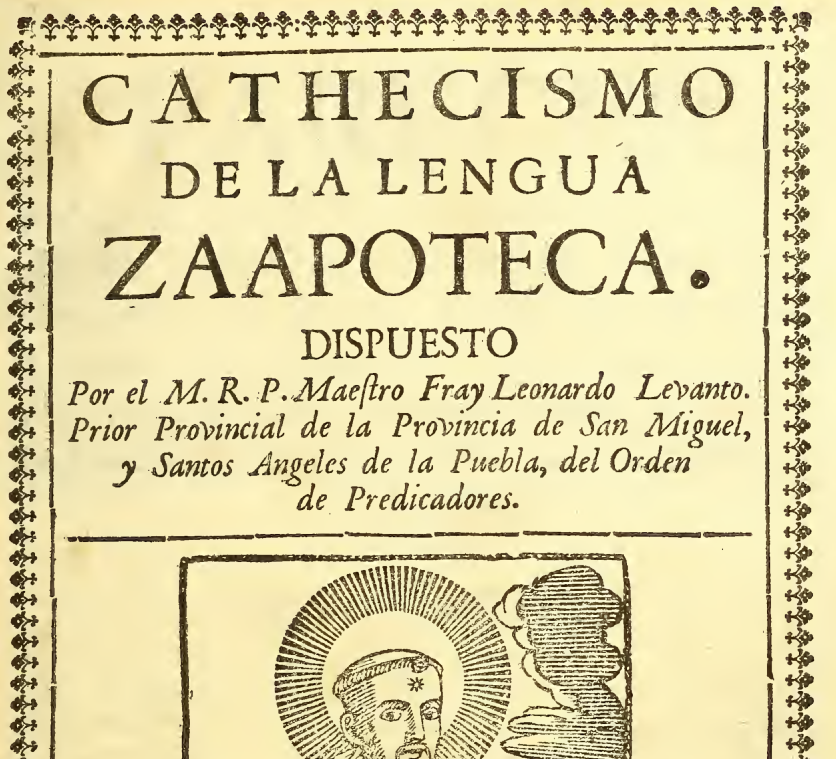
\includegraphics[scale=0.35]{Levanto1766_TitlePage} }
\caption{Levanto's (1766) \emph{Catecismo}, Title Page (Page 5)}
\label{fig:levanto1766_TitlePage}
\end{figure}

To begin we indicate the first relevant page break.  The tag for this is \hyperref[tag-sec:pb]{\texttt{<pb/>}}; notice that this is a self-closing tag.  Page break tags can take several attributes.  All \texttt{<pb/>}'s have the \hyperref[att-sec:break]{\texttt{break}} attribute, which indicates whether it is a true break or whether a word is split between the two pages.  This particular page break is indeed a break in the text, so here we use the value \texttt{"yes"}.

\texttt{<pb/>} tags also take the \hyperref[att-sec:type]{\texttt{type}} attribute.  We put two types of page beginnings at every page turn, one with \texttt{type} value \colorbox{cyan}{\texttt{"levanto"}}, indicating that the text itself changes pages, and one with value \colorbox{green}{\texttt{"pdf"}}, indicating tat the PDF scan of the text has a new page.  The \texttt{"levanto"} type has a further attribute \hyperref[att-sec:n]{\texttt{n}} which takes the value of the page number, in this case \texttt{"5"}.  The \texttt{"pdf"} type has a further attribute \hyperref[att-sec:facs]{\texttt{facs}}, which has the value of the url to the scanned image of that page of the document.

\begin{lstlisting}
<front>
	<div xml:id="levanto1" part="N" org="uniform" sample="complete">
		<head type="outline">1 [Front matter]</head>
		<div xml:id="levanto1.1" part="N" org="uniform" sample="complete">
			<head type="outline">
				1.1 [Cover of book and preliminary pages]
			</head>
			<!-- these preliminary pages have no transcription -->
			^\colorbox{cyan}{<pb break="yes" type="levanto" n="5"/>}^    
			^\colorbox{green}{<pb break="yes" type="pdf" facs="https://url/to/scan"/>}^
		</div>
	</div>
</front>
\end{lstlisting}

Now that we have begun the page, we want to begin Section 1.2.  As before we use a \texttt{<div>} with the appropriate attributes and a \texttt{<head>} with \texttt{type="outline"}.  (Here I will reduce the code to just the relevant \texttt{<div>}).

\begin{lstlisting}[escapechar=^]
<div xml:id="arte1.2" part="N" org="uniform" sample="complete">
	<head type="outline">1.2 [Title Page]</head>
</div>
\end{lstlisting}

This time we also have a heading which is printed in text, namely the title of the book, which requires a \texttt{<head>} tag with the attribute \texttt{type="levanto"}

\begin{lstlisting}
<div xml:id="levanto1.2" part="N" org="uniform" sample="complete">
	<head type="outline">1.2 [Title Page]</head>  
	^\colorbox{yellow}{<head type="levanto"></head>}^
</div>
\end{lstlisting}

Now we transcribe the text exactly as it appears in print.  Line breaks are indicated with the self-closing \hyperref[tag-sec:lb]{\texttt{<lb/>}} tag.  Images, like the woodcut on this page, can be noted in a comment.

\begin{lstlisting}
<div xml:id="levanto1.2" part="N" org="uniform" sample="complete">
	<head type="outline">1.2 [Title Page]</head>  
	<head type="levanto">
		C A T H E C I S M O
		<lb/>D E L A L E N G U A
		<lb/>Z A A P O T E C A.
		<lb/>DISPUESTO
		<lb/>Por el M. R. P.Maeftro Fray Leonardo Levanto.
		<lb/>Prior Provincial de la Provincia de San Miguel,
		<lb/>y Santos Angeles de la Puebla, del Orden
		<lb/> de Predicadores.
	</head>
	<!-- woodcut -->
</div>
\end{lstlisting}

Much of the Spanish in the title is non-standard, so we use \hyperref[tag-sec:choice]{\texttt{<choice>}} tags to provide the regularized version.  Notice that the original transcription is enclosed in the \hyperref[tag-sec:orig]{\texttt{<orig>}} tag and the regularized version is enclosed in the \hyperref[tag-sec:reg]{\texttt{<reg>}} tag.  The \texttt{<reg>} tag also takes an attribute \hyperref[att-sec:type]{\texttt{type}}, with the value of the language which is being regularized.

\begin{lstlisting}
<choice><orig>C A T H E C I S M O</orig><reg type="spanish">CATECISMO</reg></choice>
\end{lstlisting}

The final encoding the front matter so far is:

\begin{lstlisting}
<front>
	<div xml:id="levanto1" part="N" org="uniform" sample="complete"> 
		<head type="outline">1 [Front matter]</head>
		<div xml:id="levanto1.1" part="N" org="uniform" sample="complete">
			<head type="outline">
				1.1 [Cover of book and preliminary pages]
			</head>
			<!-- these preliminary pages have no transcription -->
			<pb break="yes" type="levanto" n="5"/>
			<pb break="yes" type="pdf" facs="https://url/to/scan"/>
		</div>
		<div xml:id="levanto1.2" part="N" org="uniform" sample="complete">
			<head type="outline">1.2 [Title Page]</head>  
			<head type="levanto">
				<choice><orig>C A T H E C I S M O</orig><reg type="spanish">CATECISMO</reg></choice>
				<lb/><choice><orig>D E</orig><reg type="spanish">DE</reg></choice> 
				<choice><orig>L A</orig><reg type="spanish">LA</reg></choice> 
				<choice><orig>L E N G U A</orig><reg type="spanish">LENGUA</reg></choice>
				<lb/><choice><orig>Z A A P O T E C A</orig><reg type="spanish">ZAPOTECA</reg></choice>.
				<lb/>DISPUESTO
				<lb/>Por el M. R. P.
				<choice><orig>Maeftro</orig><reg type="spanish">Maestro</reg></choice> 
				Fray Leonardo Levanto.
				<lb/>Prior Provincial de la Provincia de San Miguel,
				<lb/>y Santos Angeles de la Puebla, del Orden
				<lb/> de Predicadores.
			</head>
			<!-- woodcut -->
		</div>
	</div>
</front>
\end{lstlisting}

\subsection{Body Text of Levanto's \emph{Catecismo}}

italics with <hi>?

\begin{figure}[h]
\centerline{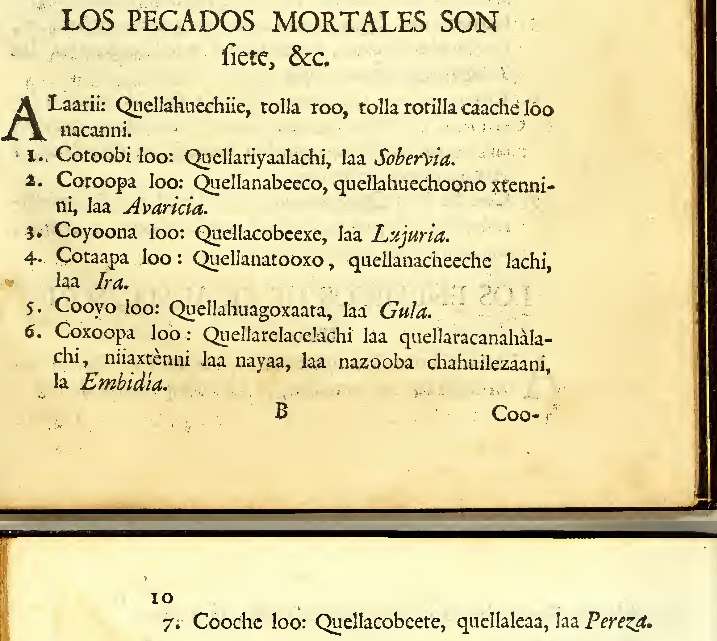
\includegraphics[scale=0.55]{Levanto1766_Page9} }
\caption{Levanto's (1766) \emph{Catecismo}, Page 9--10}
\end{figure}

As before we mark the section with an appropriate marked \hyperref[tag-sec:div]{\texttt{<div>}}.  Since this section is primarily in Zapotec, we using the \hyperref[att-sec:xml:lang]{\texttt{xml:lang}} attribute with the value \texttt{"cvz"}.\footnote{Depending on the structure of this part of the document, it may be appropriate to but the \texttt{xml:lang} tag at a higher level.}

\begin{lstlisting}
<div xml:id="levanto3.4" xml:lang="cvz">
</div>
\end{lstlisting}

We begin the section with two \hyperref[tag-sec:head]{\texttt{<head>}} marked with \hyperref[att-sec:type]{\texttt{type}} attributes, one \texttt{"outline"} and the other \texttt{"levanto"}.  Since we have marked the section as Zapotec, we use the \hyperref[att-sec:xml:lang]{\texttt{xml:lang}} attribute with the value \texttt{"es"} to indicate that the headings are in Spanish.  (Notice that ampersands are indicated using \texttt{\&amp;}, a predefined character reference.\footnote{See \url{http://www.tei-c.org/release/doc/tei-p5-doc/en/html/SG.html\#SG-er}.}

\begin{lstlisting}
<div xml:id="levanto3.4" xml:lang="cvz">
	<head type="outline" ^\colorbox{yellow}{xml:lang="es"}^>
		3.4 Los pecadores mortales
	<head>
	<head type="levanto" ^\colorbox{yellow}{xml:lang="es"}^>
		LOS PECADOS MORTALES SON
		<lb/><choice><orig>fiete</orig><reg>siete</reg></choice>
		, &amp;c.
	</head>
</div>
\end{lstlisting}

We then add the first paragraph of the body text, contained in a \hyperref[tag-sec:p]{\texttt{<p>}} tag.

\begin{lstlisting}
<div xml:id="levanto3.4" xml:lang="cvz">
	<head type="outline" xml:lang="es">
		3.4 Los pecadores mortales
	<head>
	<head type="levanto" xml:lang="es">
		LOS PECADOS MORTALES SON
		<lb/><choice><orig>fiete</orig><reg>siete</reg></choice>
		, &amp;c.
	</head>
	^\colorbox{yellow}{<p>}^
		^\colorbox{yellow}{<choice><orig>ALaarii</orig><reg type="cvz">Alaarii</reg></choice>}^
		^\colorbox{yellow}{: Quellahuechiie, tolla roo, tolla rotilla caache loo}^
		^\colorbox{yellow}{<lb/>nacanni.}^
	^\colorbox{yellow}{</p>}^
</div>
\end{lstlisting}

The next paragraph has a word in Spanish.  This is marked using the \hyperref[tag-sec:foreign]{\texttt{<foreign>}} tag with the \hyperref[att-sec:xml:lang]{\texttt{xml:lang}} attribute.

\begin{lstlisting}
<p>
	1.  Cotoobi loo: Quellariyaalachi, laa 
	^\colorbox{yellow}{<foreign xml:lang="es">}^
		<choice><orig>Sobervia</orig><reg type="spanish">Soberbia</reg></choice>
	</foreign>.
</p>
\end{lstlisting}

In the last paragraph on the page, a word is broken across two lines.  We indicate this by adding a \hyperref[att-sec:break]{\texttt{break}} attribute with the value \texttt{"no"} to the \hyperref[tag-sec:lb]{\texttt{<lb/>}} tag.  The hyphen is contained in a \hyperref[tag-sec:pc]{\texttt{<pc>}} tag with type \texttt{"hyphen"},

\begin{lstlisting}
<p>
	6.  Coxoopa loo: Quellarelacelachi laa ^\colorbox{yellow}{quellaracanahàla}^
	^\colorbox{yellow}{<pc type="hyphen">-</pc>}^
	^\colorbox{yellow}{<lb break="no"/>chi}^, niiaxtènni laa nayaa, laa nazooba chahuilezaani,
	<lb/>la <foreign xml:lang="es">Embidia</foreign>.
</p>
\end{lstlisting}

The bottom of page 9 and the top of page 10 both have forme work, which is headers and footers that are separate from the rest of the information on the page.  This information is enclosed in \hyperref[tag-sec:fw]{\texttt{<fw>}} tags described by a \hyperref[att-sec:type]{\texttt{type}} attribute.  The bottom of page nine has a signature marker ``B'', which is marked \texttt{type="sig"}, and a catchword ``Coo-'', which is marked \texttt{type="catchword"}.  After the page break, at the top of page 10, we have a page number, which is marked \texttt{type="pageNum"}.  Each \hyperref[tag-sec:fw]{\texttt{<fw>}} tag also takes the \hyperref[att-sec:place]{\texttt{place}} attribute, which describes where on the page it is located.  The \hyperref[tag-sec:hi]{\texttt{<hi>}} tag is used to indicate that this text is graphically distinct from the surrounding text.

\begin{lstlisting}
<fw ^\colorbox{yellow}{type="sig"}^ ^\colorbox{cyan}{place="bottom-center"}^>
	<hi>B</hi>
</fw>
<fw ^\colorbox{yellow}{type="catchword"}^ ^\colorbox{cyan}{place="bottom-right"}^>
	<hi>Coo<pc type="hyphen">-</pc></hi>
</fw>
<pb break="yes" type="arte" n="10"/>
<pb break="yes" type="pdf" facs="https://url/to/scan"/>
<fw ^\colorbox{yellow}{type="pageNum"}^ ^\colorbox{cyan}{place="top-left"}^>10</fw>
\end{lstlisting}

The full encoding of this section is shown below:

\begin{lstlisting}
<div xml:id="levanto3.4" xml:lang="cvz">
	<head type="outline" xml:lang="es">
		3.4 Los pecadores mortales
	<head>
	<head type="levanto" xml:lang="es">
		LOS PECADOS MORTALES SON
		<lb/><choice><orig>fiete</orig><reg>siete</reg></choice>
		, &amp;c.
	</head>
	<p>
		<choice><orig>ALaarii</orig><reg type="cvz">Alaarii</reg></choice>
		: Quellahuechiie, tolla roo, tolla rotilla caache loo
		<lb/>nacanni.
	</p>
	<p>
		1.  Cotoobi loo: Quellariyaalachi, laa <foreign xml:lang="es"><choice><orig>Sobervia</orig><reg type="spanish">Soberbia</reg></choice></foreign>.
	</p>
<!-- [snipped]  -->
	<p>
		6.  Coxoopa loo: Quellarelacelachi laa quellaracanahàla<pc type="hyphen">-</pc>
		<lb break="no"/>chi, niiaxtènni laa nayaa, laa nazooba chahuilezaani,
		<lb/>la <foreign xml:lang="es">Embidia</foreign>.
	</p>
	<fw type="sig" place="bottom-center??">
		<hi>B</hi>
	</fw>
	<fw type="catchword" place="bottom-right">
		<hi>Coo<pc type="hyphen">-</pc></hi>
	</fw>
	<pb break="yes" type="arte" n="10"/>
	<pb break="yes" type="pdf" facs="https://url/to/scan"/>
	<fw type="pageNum" place="top-left">10</fw>
	<p>
		7.  Cooche loo: Quellacobcete, quellaleaa, laa <foreign xml:lang="es">Pereza</foreign>.
	</p>
</div>
\end{lstlisting}

\subsection{Ellipsis in Cordova's \emph{Arte}} \label{sec:arte-ellipsis}

Throughout the \emph{Arte}, Cordova frequently uses ellipsis to conserve space.  This happens where there are multiple CVZ words that share a root.  For example, he list two CVZ words for twenty-two, \emph{callebitopa} and \emph{callebicato}, but lists this as \emph{callebitopa.l.cato}, eliding the second \emph{callebi} and using \emph{l}, the abbreviation for Latin \emph{vel} `or'.

\begin{figure}[h]
\centerline{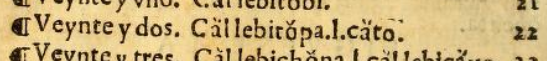
\includegraphics[scale=0.70]{Arte_Page99v} }
\caption{Cordova's (1578) \emph{Arte}, Page 99v}
\end{figure}

To encode this we use the \hyperref[tag-sec:gap]{\texttt{<gap>}} tag, which indicates letters which are supposed to be in the text but are not actually represented on the page.  The \texttt{<gap>} tag takes a \hyperref[att-sec:reason]{\texttt{reason}} attribute and optionally an \hyperref[att-sec:agent]{\texttt{agent}} attribute.  In this case we use the \texttt{reason="ellipsis"}.  (In another case we might say, for example, \texttt{reason="illegible"}).  This line is encoded as below:

\begin{lstlisting}
<p>
	<pc>^\P^</pc>
	<choice>
		<orig>Veynte y dos</orig>
		<reg type="spanish">Veintid^\'{o}^s</reg>
	</choice>.
	<foreign xml:lang="cvz">Callebitopa</foreign>. 
	<foreign xml:lang="lat">
		<choice><abbr>l</abbr><expan>vel</expan></choice>
	</foreign>. 
	<foreign xml:lang="cvz">
		^\colorbox{yellow}{<gap reason="ellipsis">Callebi</gap>}^cato
	</foreign>. 22
</p>
\end{lstlisting}

\subsection{Parallel Text in Levanto's \emph{Catecismo}}

\begin{figure}[h]
\centerline{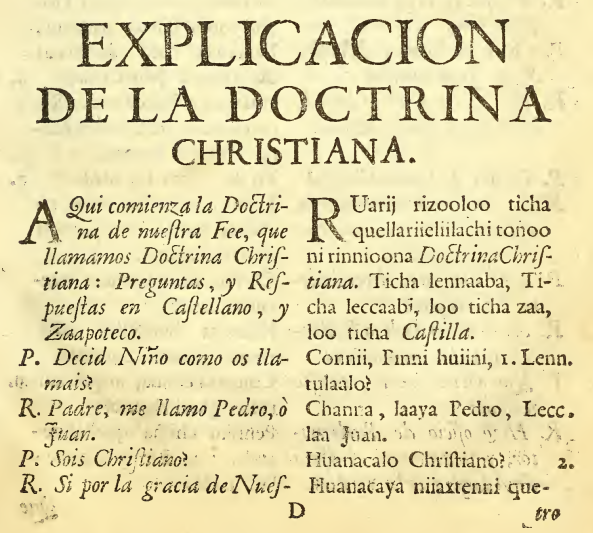
\includegraphics[scale=0.55]{Levanto1766_Page17} }
\caption{Levanto's (1766) \emph{Catecismo}, Page 17}
\end{figure}

\begin{figure}[h]
\centerline{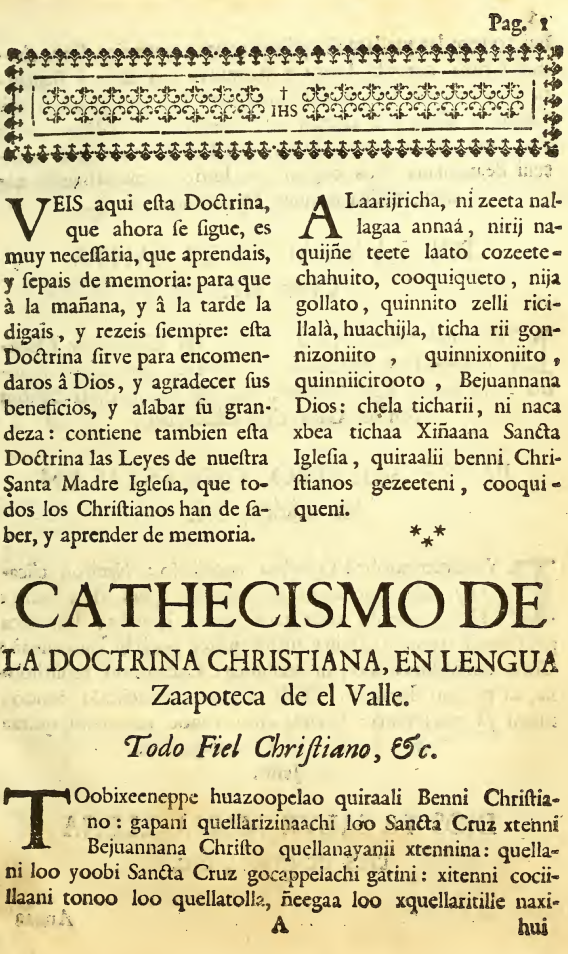
\includegraphics[scale=0.4]{Levanto1766_Page1Full} }
\caption{Levanto's (1766) \emph{Catecismo}, Page 1}
\end{figure}



\end{document}